\documentclass[conference]{IEEEtran}
\IEEEoverridecommandlockouts
% The preceding line is only needed to identify funding in the first footnote. If that is unneeded, please comment it out.
\usepackage{cite}
\usepackage{amsmath,amssymb,amsfonts}
\usepackage{algorithmic}
\usepackage{graphicx}
\usepackage{textcomp}
\usepackage{xcolor}
\usepackage{url}
\usepackage{subfig}
\usepackage{float}
\usepackage{hyperref}
\usepackage{tikz}
\usetikzlibrary{shapes.geometric, arrows.meta, positioning}


\def\BibTeX{{\rm B\kern-.05em{\sc i\kern-.025em b}\kern-.08em
    T\kern-.1667em\lower.7ex\hbox{E}\kern-.125emX}}

\begin{document}

\title{Embedded Linux and Real-Time Operating System Development for Internet of Things Applications}


\author{
\IEEEauthorblockN{Youssef Khaled Omar Mahmoud}

\IEEEauthorblockA{
Department of Electrical, Electronic and Communication Engineering\\
Faculty of Engineering, Cairo University\\
Giza, Egypt\\
\texttt{youefkh05@gmail.com}\\
ORCID: \texttt{0009-0005-5807-4381}
}
}

\maketitle

\begin{abstract}
This paper presents the work completed during the IoT Summer Research Internship 2026 at the Nanoelectronics Integrated Systems Center (NISC), Nile University. The internship focused on embedded systems, Internet of Things (IoT), and real-time operating systems through a series of hands-on tasks. The developed solutions demonstrated communication between embedded devices and cloud services while providing practical experience in embedded software development, cloud technologies, wireless communication, and system integration.
\end{abstract}


\begin{IEEEkeywords}
Internet of Things (IoT), Embedded Systems, Raspberry Pi, Embedded Linux, TI-RTOS, CC1352P1 LaunchPad, MQTT, HTTP, InfluxDB, Grafana, UART, Bluetooth, Zigbee.
\end{IEEEkeywords}


\section{Introduction}

The Nile University Summer Research Internship 2026 provided an opportunity to gain practical experience in embedded systems, Internet of Things (IoT), and real-time software development through a series of hands-on engineering tasks. The internship emphasized applying theoretical knowledge to real-world embedded applications while introducing modern software and communication technologies widely used in industry.

Throughout the internship, three major technical areas were explored. The first focused on Embedded Linux development using the Raspberry Pi, where Python was employed to interface with hardware peripherals and implement different GPIO control techniques. The second addressed the design of an end-to-end IoT system by transmitting sensor measurements from edge devices to cloud services using both HTTP and MQTT communication protocols. The collected data were stored in a time-series database and visualized through a real-time monitoring dashboard. Finally, the internship introduced real-time embedded software development using TI-RTOS on the Texas Instruments CC1352P1 LaunchPad, where multiple concurrent tasks including LED control, Bluetooth communication, Zigbee communication, and UART-based communication with the Raspberry Pi were implemented.

In addition to software implementation, the internship emphasized understanding the design trade-offs between different communication protocols and software architectures. The progression from basic hardware interfacing to cloud connectivity and finally to multitasking embedded systems provided a comprehensive view of modern IoT system development.

This report summarizes the assigned tasks, describes the methodologies followed during implementation, presents the achieved results, and discusses the technical knowledge and practical skills acquired throughout the internship.

\section{Assigned Tasks}

The internship activities were organized progressively over several weeks, with each stage building upon the knowledge and skills acquired in the previous one. \cite{repo}

\subsection*{Week 1: Embedded Linux and Raspberry Pi}
\begin{itemize}
    \item Raspberry Pi development using Embedded Linux.
    \item Python programming for hardware interfacing.
    \item GPIO programming and sensor interfacing.
\end{itemize}

\subsection*{Weeks 2--3: Internet of Things (IoT)}
\begin{itemize}
    \item Cloud communication using HTTP.
    \item Cloud communication using MQTT.
    \item Data storage using InfluxDB.
    \item Data visualization using Grafana.
\end{itemize}

\subsection*{Weeks 3--4: Real-Time Operating Systems (RTOS)}
\begin{itemize}
    \item Real-Time Operating System (RTOS) programming.
    \item Bluetooth communication.
    \item Zigbee communication.
    \item UART-over-USB communication.
    \item Integration between the RTOS microcontroller and the Raspberry Pi.
\end{itemize}

\section{Brief Description of Assigned Tasks}

The internship was organized into three major technical tasks that progressively introduced embedded systems, Internet of Things (IoT), and real-time operating systems (RTOS). Each task combined theoretical concepts with practical implementation, allowing the development of complete embedded applications and their integration into an end-to-end IoT system. \cite{repo}

\subsection{Raspberry Pi Development}

\subsubsection{Objective}

The objective of this task was to develop a solid foundation in software development on Embedded Linux while learning the fundamentals of hardware interfacing using the Raspberry Pi. The work progressed from C programming exercises to GPIO-based control applications, providing practical experience in software design, Linux development, and interaction with external hardware peripherals.

\subsubsection{Task 2.1 -- C Programming Fundamentals}

The first stage focused on strengthening programming skills using the C language within the Raspberry Pi Linux environment. The implemented application solved the Emirp Number problem, where prime numbers whose digit-reversed values are also prime were identified within a user-defined range.

The program was developed using a modular design by separating the functionality into helper functions responsible for primality testing and digit reversal. Dynamic memory allocation was employed to store the resulting Emirp pairs, while structures were used to organize the associated data, including the prime number, its inverse, and the numerical difference between them. Input validation was also incorporated to detect invalid ranges and incorrect user entries before executing the algorithm.

This task provided practical experience with:

\begin{itemize}
    \item Programming in C under Embedded Linux.
    \item Modular software development using functions.
    \item Structure-based data organization.
    \item Dynamic memory allocation using \texttt{malloc()}.
    \item Input validation and error handling.
    \item Compilation and execution using the GNU Compiler Collection (GCC).
\end{itemize}

The overall workflow of the developed Emirp application is illustrated in Figure~\ref{fig:emirp_flow}. The program begins by validating the user inputs, allocates memory dynamically for storing valid Emirp pairs, iterates through the specified range to identify qualifying numbers, and finally computes statistical information before displaying the results. Example executions are presented in Figure~\ref{fig:prime_examples}, while representative input-output cases are summarized in Table~\ref{tab:emirp_examples}.


\begin{table}[ht]
\caption{Representative execution scenarios of the Emirp number application.}
\label{tab:emirp_examples}
\centering
\begin{tabular}{|c|p{0.58\columnwidth}|}
\hline
\textbf{Input Range} & \textbf{Observed Result} \\ \hline
11 -- 100 & Emirp pairs successfully identified and summarized. \\ \hline
101 -- 500 & Larger set of Emirp numbers processed correctly. \\ \hline
50 -- 10 & Invalid range detected and an appropriate error message displayed. \\ \hline
Negative or even inputs & Input validation rejected invalid values before execution. \\ \hline
\end{tabular}
\end{table}


Table~\ref{tab:emirp_examples} summarizes representative execution scenarios of the developed application.


\begin{figure}[H]
\centering
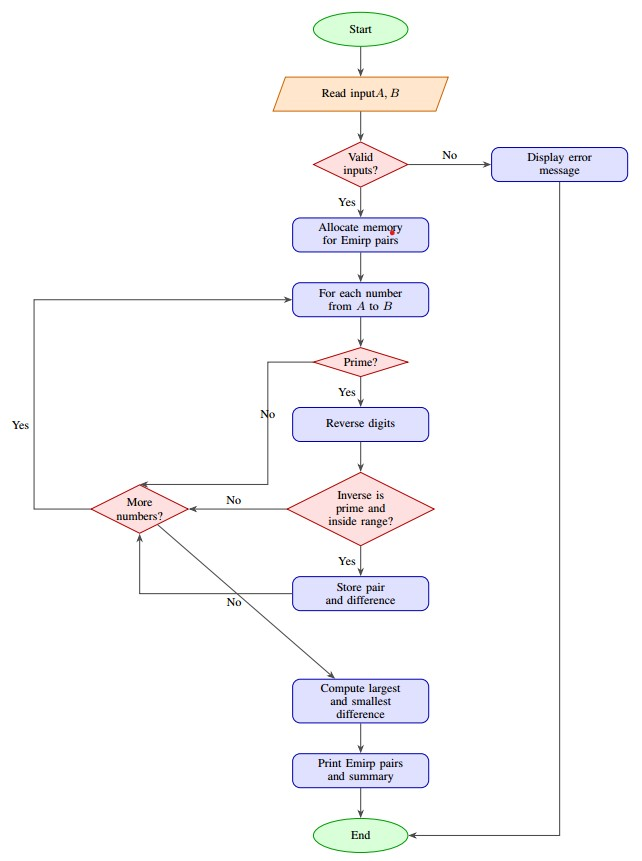
\includegraphics[width=0.9\columnwidth]{../Tasks/Task2/T2_prime_Flow.jpeg}
\caption{Flowchart of the implemented Emirp number detection algorithm.}
\label{fig:emirp_flow}
\end{figure}


While Figure~\ref{fig:prime_examples} presents sample terminal outputs obtained during testing.


\begin{figure}[H]
\centering

\subfloat[Typical execution.]{
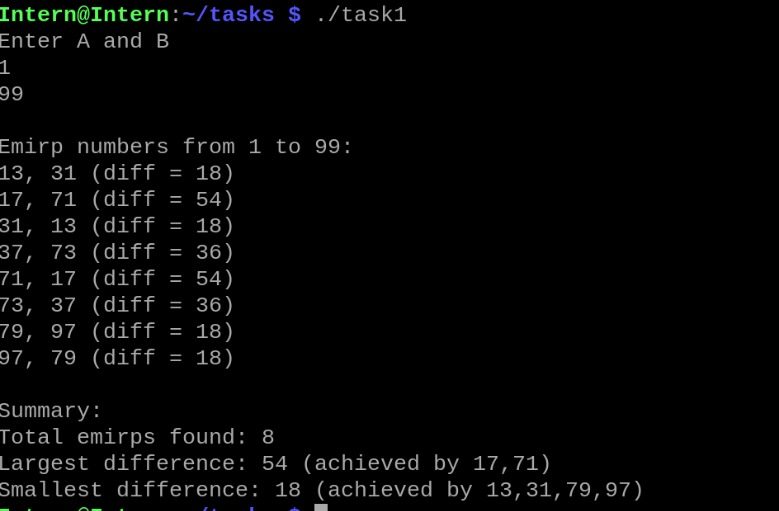
\includegraphics[width=.47\columnwidth]{../Tasks/Task2/T2_prime_test.jpeg}}
\hfill
\subfloat[Small range.]{
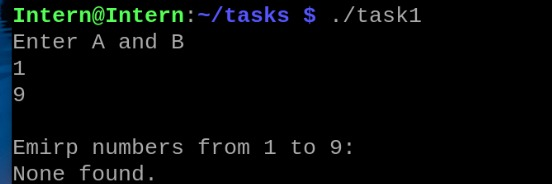
\includegraphics[width=.47\columnwidth]{../Tasks/Task2/T2_prime_small.jpeg}}

\vspace{0.4em}

\subfloat[Large range.]{
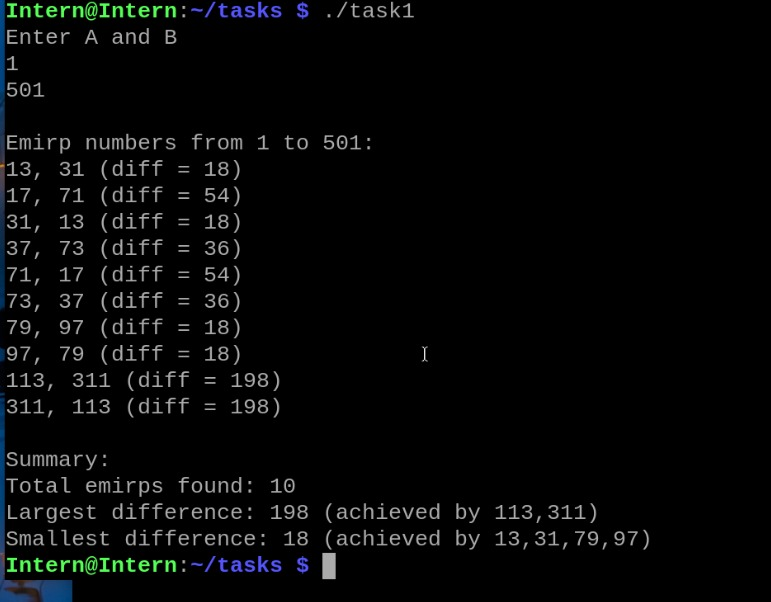
\includegraphics[width=.47\columnwidth]{../Tasks/Task2/T2_prime_large.jpeg}}
\hfill
\subfloat[Invalid input.]{
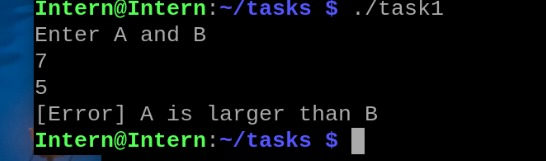
\includegraphics[width=.47\columnwidth]{../Tasks/Task2/T2_prime_test_erro.jpeg}}

\caption{Terminal outputs demonstrating successful execution and input validation of the Emirp number application.}
\label{fig:prime_examples}

\end{figure}

\subsubsection{Task 2.2 -- Embedded Linux and GPIO Programming}

The second stage introduced hardware interfacing using the Raspberry Pi GPIO pins. Python was used to control LEDs and read the state of a push button through the GPIO interface provided by the Linux operating system.

Three different software approaches were implemented for LED control:

\begin{itemize}
    \item \textbf{Delay-based control}, where software delay loops generated the blinking period.
    \item \textbf{Timer-based control}, where timing mechanisms were used to improve execution accuracy.
    \item \textbf{Interrupt-based control}, where GPIO interrupts enabled immediate response to button presses without continuous polling.
\end{itemize}

These implementations demonstrated how different software architectures influence processor utilization, timing accuracy, and system responsiveness while using identical hardware.

\subsubsection{Outcomes}

\begin{figure}[H]
\centering
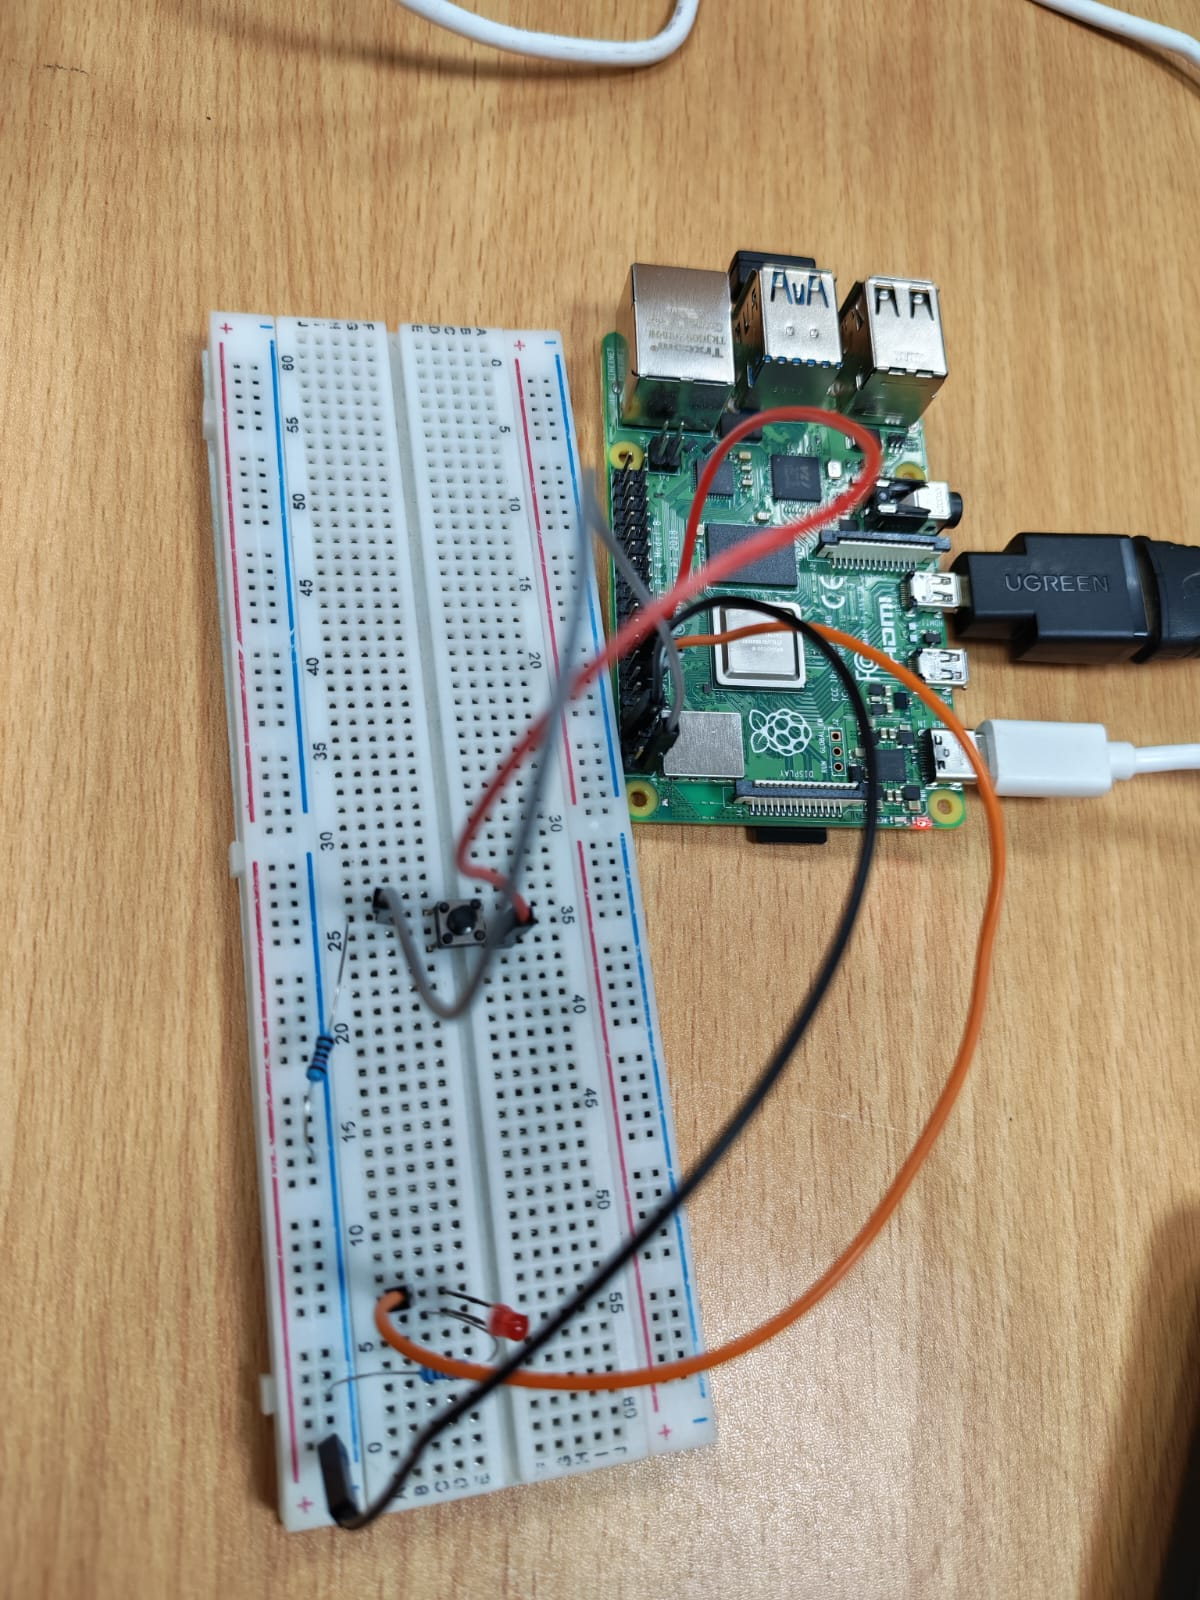
\includegraphics[width=0.9\columnwidth]{../Tasks/Task3/T3_Button.jpeg}
\caption{GPIO-based LED control implemented on the Raspberry Pi.}
\label{fig:led}
\end{figure}

Example executions of the developed C application are presented in Figure~\ref{fig:prime_examples}, while Figure~\ref{fig:led} illustrates the GPIO-based LED control implemented on the Raspberry Pi.

The Raspberry Pi tasks successfully demonstrated both software development and embedded hardware interfacing. The C programming exercise reinforced fundamental programming concepts, including modular design, dynamic memory management, and algorithm implementation. The GPIO applications provided practical experience in controlling external peripherals, implementing event-driven programming techniques, and comparing different software control methodologies. Figure~\ref{fig:led} illustrates the implemented GPIO-based LED control setup.

\section*{Acknowledgment}

The author would like to express sincere gratitude to the Nile University Research Office for offering the opportunity to participate in the 2026 IoT Summer Research Internship Program.

Special thanks are extended to   \href{https://www.nu.edu.eg/academic-staff/dr-ahmed-soltan}{Prof. Ahmed Soltan}, Director of the Nanoelectronics Integrated Systems Center (NISC), for providing this valuable opportunity, his continuous support, and for taking the time to listen to and discuss our feedback throughout the internship.

The author also gratefully acknowledges the guidance and supervision of Eng. Salma, Eng. Omar, and Eng. Ahmed, whose technical support, constructive feedback, and mentorship were invaluable throughout the internship.

\begin{thebibliography}{99}

\bibitem{repo}
Y. K. Omar,
``NU-IoT-Research-Intern,''
GitHub repository, 2026.
Available:
\url{https://github.com/youefkh05/NU-IoT-Research-Intern}

\bibitem{videos}
Y. K. Omar,
``NU IoT Research Internship Task Demonstrations,''
Google Drive, 2026.
Available: \href{https://drive.google.com/drive/folders/1mi1f_lU7xuAddAbGfxgAJMQLgRbdzmwu?usp=sharing}{Google Drive Link}

\end{thebibliography}

\end{document}
